\documentclass[english]{article}
\usepackage{graphicx}
\usepackage{amsmath}
\usepackage{hyperref}
\usepackage{setspace}
\usepackage{apacite}
\usepackage{hyperref}
\usepackage[sort]{natbib}
\usepackage{pxfonts}
\usepackage[utf8]{inputenc}
\usepackage[left=1in,right=1in,top=1in,bottom=1in]{geometry}
\usepackage[left]{lineno}
\usepackage{soul}
\linenumbers


\title{High-level cognition is supported by at least second order
  dynamic correlations in neural activity patterns}

\author{Lucy L. W. Owen$^1$, Thomas H. Chang$^{1,2}$, and\
  Jeremy R. Manning\textsuperscript{$1, \dagger$}\\
  [0.1in]$^1$Department of Psychological and Brain
  Sciences,\\Dartmouth
  College, Hanover, NH\\
  $^3$Amazon.com, Seattle, WA\\
  \textsuperscript{$\dagger$}Address correspondence to
  jeremy.r.manning@dartmouth.edu}


\begin{document}
\maketitle


\begin{abstract}
  Our thoughts arise from coordinated patterns of interactions between
  brain structures that change with our ongoing experiences.
  High-order dynamic correlations in brain activity patterns reflect
  different subgraphs of the brain's connectome that display
  homologous lower-level dynamic correlations.  We tested the
  hypothesis that high-level cognition is supported by high-order
  dynamic correlations in brain activity patterns.  We developed an
  approach to estimating high-order dynamic correlations in timeseries
  data, and we applied the approach to neuroimaging data collected as
  human participants either listened to a ten-minute story or a
  temporally scrambled version of the story, or underwent a resting
  state scan.  We trained across-participants pattern classifiers to
  decode (in held-out data) when in the session each activity snapshot
  was collected.  We found that classifiers trained to decode from
  high-order dynamic correlations yielded better performance on data
  collected as participants listened to the (unscrambled) story.  By
  contrast, classifiers trained to decode data from scrambled versions
  of the story or during the resting state scan yielded the best
  performance when they were trained using first-order dynamic
  correlations or raw activity patterns.  We suggest that as our
  thoughts become more complex, they are supported by higher-order
  patterns of dynamic network interactions throughout the brain.
\end{abstract}

\doublespacing

\section*{Introduction}
A central goal in cognitive neuroscience is to elucidate the
\textit{neural code}: the mapping between (a) mental states or
cognitive representations and (b) neural activity patterns. One means
of testing models of the neural code is to ask how accurately that
model is able to ``translate'' neural activity patterns into known (or
hypothesized) mental states or cognitive
representations~\citep[e.g.,][]{HaxbEtal01, NormEtal06, TongPrat12,
  MitcEtal08a, KamiTong05, NishEtal11, PereEtal18, HuthEtal12,
  HuthEtal16}.  Training decoding models on different types of neural
features can also help to elucidate which specific aspects of neural
activity patterns are informative about cognition-- and, by extension,
which types of neural activity patterns might comprise the neural
code.  For example, prior work has used region of interest analyses to
estimate the anatomical locations of specific neural
representations~\citep[e.g.,][]{EtzeEtal09}, or to compare the
relative contributions to the neural code of multivariate activity
patterns versus patterns of dynamic correlations between neural
activity patterns~\citep[e.g.,][]{MannEtal18, FongEtal19}.  An
emerging theme in this literature is that cognition is mediated by
complex dynamic interactions between brain
structures~\citep{SporHone06, BassEtal06, Turk13, DemeEtal19}.

Studies of the neural code to date have primarily focused on
univariate or multivariate neural patterns~\cite[for review
see][NormEtal06], or (more recently) on patterns of dynamic
first-order correlations~\citep[i.e., interactions between pairs of
brain structures;][]{MannEtal18, FongEtal19}.  We wondered what the
future of this line of work might hold.  For example, is the neural
code mediated by higher-order interactions between brain structures?
Second-order correlations reflect \textit{homologous} patterns of
correlation.  In other words, if the changing patterns of correlations
between two regions, $A$ and $B$, are similar to those between two
other regions, $C$ and $D$, this would be reflected in the
second-order correlations between ($A$--$B$) and ($C$--$D$).  In this
way, second-order correlations identify similarities and differences
between subgraphs of the brain's connectome.  Analogously, third-order
correlations reflect homologies between second-order correlations--
i.e., homologous patterns of homologous interactions between brain
regions.  More generally, higher-order correlations reflect homologies
between patterns of lower-order correlations.  We can then ask: which
``orders'' of interaction are most reflective of high-level cognitive
processes?

Another central question pertains to the extent to which the neural
code is carried by activity patterns that directly reflect ongoing
cognition~\citep[e.g., following][]{HaxbEtal01, NormEtal06}, versus
the dynamic properties of the network structure itself, independent of
specific activity patterns in any given set of regions~\citep[e.g.,
following][]{BassEtal06}.  For example, graph theoretic measures such
as centrality and degree~\citep{BullSpor09} may be used to estimate
how a given brain structure is ``communicating'' with other
structures, independently of the specific neural representations
carried by those structures.  If one considers a brain region's graph
theoretic position in the network (e.g., its eigenvector centrality)
as a dynamic property, one can compare how the positions of different
regions are correlated, and/or how those patterns of correlations change
over time.  We can also compute higher-order patterns in these
correlations to characterize homologous subgraphs in the connectome
that display similar changes in their constituent brain structures'
interactions with the rest of the brain.

To gain insights into the above aspects of the neural code, we
developed a computational framework for estimating dynamic high-order
correlations in timeseries data. This framework provides an important
advance, in that it enables us to examine patterns in higher-order
correlations that are computationally intractable to estimate via
conventional methods.  Given a multivariate timeseries, our framework
provides timepoint-by-timepoint estimates of the first-order
correlations, second-order correlations, and so on (up to tenth-order
correlations in this manuscript).  Our approach combines a
kernel-based method for computing dynamic correlations in timeseries
data with a dimensionality reduction step that projects the resulting
dynamic correlations into a low-dimensional space.  We explored two
dimensionality reduction approaches: principle components
analysis~\citep[PCA;][]{Pear01}, which preserves an approximately invertable
transformation back to the original data; and a second non-invertible
algorithm that explored patterns in eigenvector
centrality~\citep{Land95}.  This latter approach characterizes
correlations between each feature dimension's relative
\textit{position} in the network in favor of the specific activity
histories of different features.

We validated our approach using synthetic data where the underlying
correlations were known.  We then applied our framework to a
neuroimaging dataset collected as 125 participants listened to either
an audio recording of a ten-minute story or a temporally scrambled
version of the story, or underwent a resting state
scan~\citep{SimoEtal16}.  We used a subset of the data to train
across-participant classifiers to decode listening times using a blend
of neural features (comprising neural activity patterns, as well as
different orders of correlations between those patterns that were
inferred using our computational framework).  We found that both the
PCA-based and eigenvector centrality-based approaches yielded neural
patterns that could be used to decode accurately.  Both approaches
also yielded the best decoding accuracy for data collected during
(intact) story listening when high-order (PCA:
second-order; eigenvector centrality: fourth-order) dynamic
correlation patterns were included as features.  When we trained
classifiers on the scambled stories or resting state data, only
lower-order dynamic patterns were informative to the decoders.  Taken
together, our results indicate that high-level cognition is supported
by high-order dynamic patterns of communication between brain
structures.

\section*{Methods}
Our general approach to comprises four general steps.  First, we
derive a kernel-based approach to computing dynamic pairwise
correlations in a multivariate timeseries.  Next, we apply a
dimensionality reduction step to \textbf{JRM STOPPED HERE}


A major challenge to studying such patterns is that typically neither
the correlations nor the hierarchical organizations of those
correlations may be directly observed.  Rather, these fundamental
properties must be inferred indirectly by examining the observable
parts of the system-- e.g., the behaviors of the individual units of
that system.  Here we propose a series of mathematical operations that may be used to approximate dynamic correlations at a range of scales (i.e., orders of interaction).

There are two basic steps to our approach (Fig.~\ref{fig:methods_fig}).  In the first step, we take
a number-of-timepoints ($T$) by number-of-features ($F$)
\textit{matrix of observations} ($\mathbf{X}$) and we return a $T$ by
$\frac{F^2 - F}{2}$ \textit{matrix of dynamic correlations}
($\mathbf{Y}$).  Here $\mathbf{Y_0}$ describes, at each moment, how
all of the features (columns of $\mathbf{X}$) are inferred to be
interacting.  (Since the interactions are assumed to be non-recurrent
and symmetric, only the upper triangle of the full correlation matrix
is computed.)  In the second step, we project $\mathbf{Y_0}$ onto an
$F$-dimensional space, resulting in a new $T$ by $F$ matrix
$\mathbf{Y_1}$.  Note that $\mathbf{Y_1}$ contains information about
the correlation dynamics present in $\mathbf{X}$, but represented in a
compressed number of dimensions.  By repeatedly applying these two
steps in sequence, we can examine and explore higher order dynamic
correlations in $\mathbf{X}$.

\subsection*{Dynamic correlations}
Given a matrix of observations, we can compute the (static)
correlations between any pair of observations, $\mathbf{X}_i$ and
$\mathbf{X}_j$ using:
\begin{align}
  \mathrm{corr}(\mathbf{X}_i, \mathbf{X}_j) &= \frac{\sum_{t=1}^T \left(\mathbf{X}_i(t)
                                              -
                                              \bar{\mathbf{X}_i}\right) \left(\mathbf{X}_j(t)
                                              -
                                              \bar{\mathbf{X}_j}\right)}{\sqrt{\sum_{t=1}^T
                                              \sigma^2_{\mathbf{X}_i} 
                                              \sigma^2_{\mathbf{X}_j}}},~\mathrm{where}\\\label{eqn:corr}
  \bar{\mathbf{X}_k} &= \sum_{t=1}^T
                       \mathbf{X}_k(t),~\mathrm{and}\\
  \sigma^2_{\mathbf{X}_k} &= \sum_{t=1}^T \left( \mathbf{X}_k -
                            \bar{\mathbf{X}_k} \right)^2 
\end{align}

We can generalize this formula to compute time-varying correlations by
incorporating a \textit{weight function} that takes a time $t$ as input,
and returns how much the observed data every timepoint (including $t$)
contribute to the correlations at time $t$ (Fig.~\ref{fig:weights}).
\begin{figure}
  \centering
  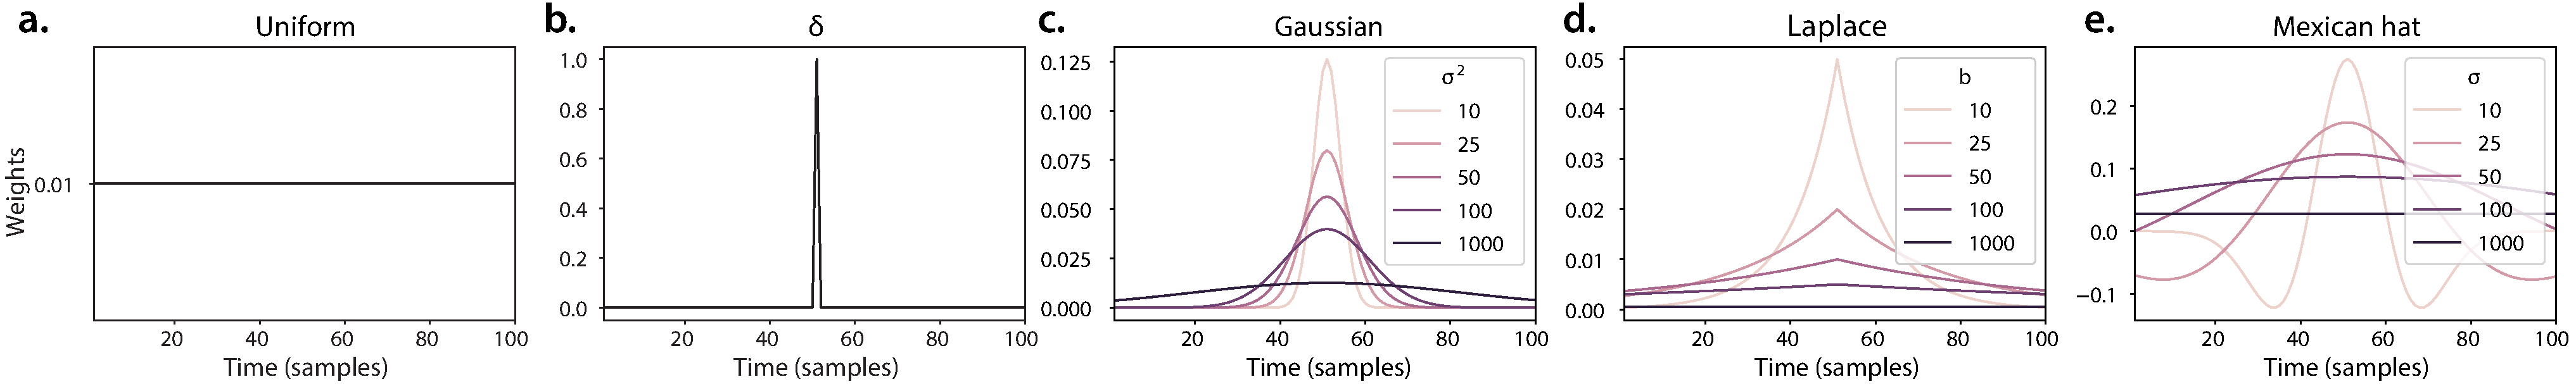
\includegraphics[width=\textwidth]{figs/kernels}
  \caption{\textbf{Examples of time-varying weights.  Each panel
      displays per-timepoint weights at $t = 50$, evaluated for 100
      timepoints ($1, ..., 100$).  a. Uniform weights.} The weights
    are timepoint-invariant; observations at all timepoints are
    weighted equally, and do not change as a function of $t$.  This is
    a special case of weight function that reduces dynamic
    correlations to static correlations.  \textbf{b. Dirac delta
      function.} Only the observation at timepoint $t$ is given weight
    (of 1), and weights for observations at all other timepoints are
    set to 0.  \textbf{c. Gaussian weights.} Each observation's
    weights fall off in time according to a Gaussian probability
    density function centered on $\mu = t$.  Weights derived using
    several different example variance parameters ($\sigma^2$ are
    displayed.  \textbf{d. Laplace weights.}  Each observation's
    weights fall off in time according to a Laplace probability
    density function centered on $\mu = t$.  Weights derived using
    several different example scale parameters ($b$) are displayed.
    \textbf{e. Mexican hat (Ricker wavelet) weights.}  Each
    observation's weights fall off in time according to a Ricker
    wavelet centered on $t$.  This function highlights the
    \textit{contrasts} between local versus surrounding activity
    patterns in estimating dynamic correlations. Weights derived using
    several different example width parameters ($\sigma$) are
    displayed.  }
  \label{fig:weights}
\end{figure}

Given a weight function $w(t)$ for timepoint $t$, evaluated at
timepoints in the interval $\left[ 1, ..., T \right]$, we can extend the static correlation formula
in Equation~\ref{eqn:corr} to reflect an \textit{instantaneous
  correlation} at timepoint $t$:
\begin{align}
  \mathrm{timecorr}(\mathbf{X}_i, \mathbf{X}_j, t) &= \frac{\sum_{t=1}^T \left(\mathbf{X}_i(t)
                                              -
                                              \widetilde{\mathbf{X}}_i(t)\right) \left(\mathbf{X}_j(t)
                                              -
                                              \widetilde{\mathbf{X}}_j(t)\right)}{\sqrt{\sum_{t=1}^T
                                              \widetilde{\sigma}^2_{\mathbf{X}_i}(t) 
                                              \widetilde{\sigma}^2_{\mathbf{X}_j}}(t)},~\mathrm{where}\\\label{eqn:timecorr}
  \widetilde{\mathbf{X}}_k(t) &= \sum_{i=1}^T
                       w(t, i)\mathbf{X}_k(i),\\
  \widetilde{\sigma}^2_{\mathbf{X}_k}(t) &= \sum_{i=1}^T \left( \mathbf{X}_k(i) -
                            \widetilde{\mathbf{X}}_k(t) \right)^2,
\end{align}
and $w(t, i)$ is shorthand for $w(t)$ evaluated at timepoint $i$.
Equation~\ref{eqn:timecorr} may be used to estimate the instantaneous
correlations between every pair of observations, at each timepoint
(i.e., $\mathbf{Y}$).

\subsubsection*{Inter-subject dynamic correlations}
Equation~\ref{eqn:timecorr} provides a means of taking a single
observation matrix, $\mathbf{X}$ and estimating the dynamic
correlations from moment to moment, $\mathbf{Y}$.  Suppose that one
has access to a set of multiple observation matrices that reflect the
same phenomenon.  For example, one might collect neuroimaging data
from several experimental participants, as each participant performs
the same task (or sequence of tasks).  Let $\mathbf{X}_1$,
$\mathbf{X}_2$, ..., $\mathbf{X}_P$ reflect the $T$ by $F$ observation
matrices for each of $P$ participants in an experiment.  We can use
\textit{inter-subject functional connectivity}~\citep[ISFC;
][]{SimoEtal16} to compute the degree of stimulus-driven correlations
reflected in the multi-participant dataset at a given timepoint $t$
using:
\begin{align}
\bar{\mathbf{C}}(t) = M\left(R\left(\frac{1}{2P} \sum_{i=1}^P
  Z\left(Y_i(t)\right)^\mathrm{T} + Z\left(Y_i,(t)\right)\right)\right),
\end{align}
where $M$ extracts and vectorizes the diagonal and upper triangle of a symmetric
matrix, $Z$ is the Fisher $z$-transformation~\citep{Zar10}:
\begin{align}
Z(r) = \frac{\log(1+r) - \log(1-r)}{2}
\end{align}
$R$ is the inverse of $Z$:
\begin{align}
R(z) = \frac{\exp(2z - 1)}{\exp(2z + 1)},
\end{align}
and $\mathbf{Y}_i(t)$ denotes the correlation matrix
(Eqn.~\ref{eqn:corr}) between each column of $\mathbf{X}_i$ and each
column of the average observations from all \textit{other}
participants, $\bar{\mathbf{X}}_{ \backslash i}$:
\begin{align}
  \bar{\mathbf{X}}_{ \backslash i} = R\left(\frac{1}{P-1}\sum_{i \in
  \backslash i} Z\left( \mathbf{X}_i \right) \right),
\end{align}
where $ \backslash i$ denotes the set of all participants other than
participant $i$. In this way, the $T$ by $\left( \frac{F^2 - F}{2}
  + F \right)$
matrix $\bar{\mathbf{C}}$ is the time-varying extension of the ISFC
approach developed by \cite{SimoEtal16}.

\subsection*{Higher-order correlations}
Given a timeseries of dynamic correlations (e.g., obtained using
Eqn.~\ref{eqn:timecorr}), higher-order correlations reflect the
dynamic correlations between columns of $\mathbf{Y}$.  Given unlimited
computing resources, one could use repeated applications of
Equation~\ref{eqn:timecorr} to estimate these higher-order
correlations (i.e., substituting in the previous output, $\mathbf{Y}$,
for the input, $\mathbf{X}$ in the equation).  However, because each
output $\mathbf{Y}$ has $\mathcal{O}(F^2)$ columns relative to $F$ columns in
the input $\mathbf{X}$, the output of Equation~\ref{eqn:timecorr}
grows with the square of the number of repeated applications (total
cost of computing $n$\textsuperscript{th} order correlations is
$\mathcal{O}(F^{2n})$ for $n \in \mathcal{J}, n > 0$).  When $F$ or $n$ is large,
this approach quickly becomes intractable.

To make progress in computing $\mathbf{Y_{n+1}}$, we can approximate
$\mathbf{Y}_n$ by computing an $\mathcal{O}(F)$-dimensional embedding of
$\mathbf{Y}_n$, termed $\hat{\mathbf{Y}}_n$, and then we can apply
Equation~\ref{eqn:timecorr} to $\hat{\mathbf{Y}}_n$ rather than
directly to $\mathbf{Y}_n$.  This enables us to maintain $\mathcal{O}(n)$
scaling with respect to $n$, rather than exponential scaling via the
direct approach.

\begin{figure}
  \centering
  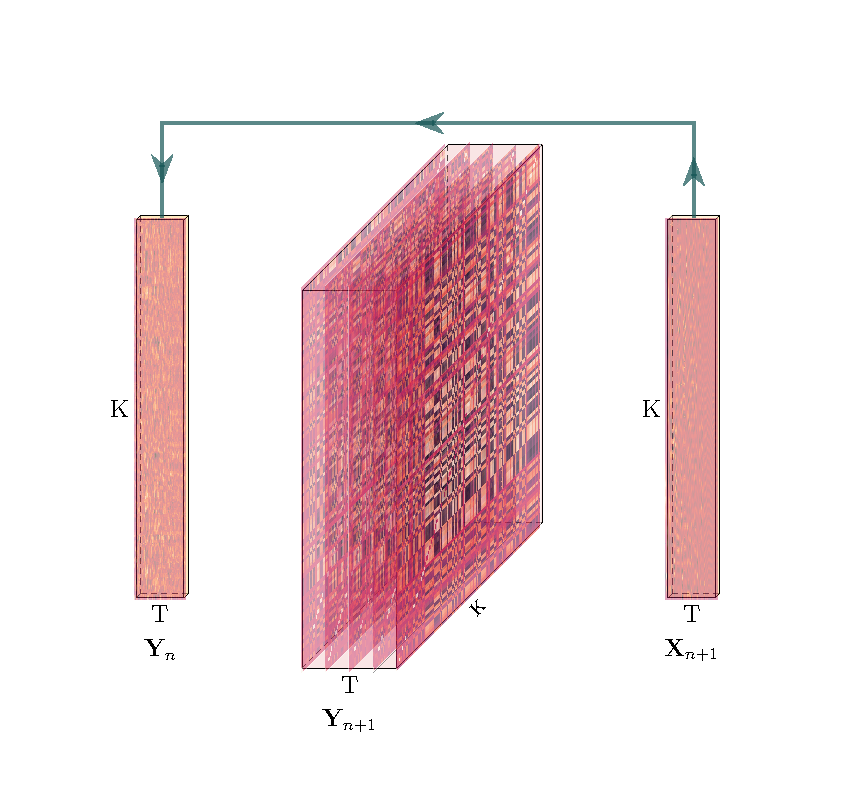
\includegraphics[width=0.5\textwidth]{figs/methods_fig}
  \caption{\textbf{Computing higher order correlations. } Dynamic
    correlations
  are computed then approximated to the same size as original data
  using dimensionality reduction.
  This process is repeated, and can be used to compute up to any
  arbitrary order with compuations scaling linearly (as opposed to exponentially) with order. }
  \label{fig:methods_fig}
\end{figure}


There are many possible methods for computing $\hat{\mathbf{Y}}_n$
from $\mathbf{Y}_n$, including traditional dimensionality reduction
approaches and graph theory based approaches as described next.  In the
\textit{Discussion} section we elaborate on other potential approaches.

\subsubsection*{Dimensionality reduction-based approaches to computing
  $\hat{\mathbf{Y}}_n$}

Commonly used dimensionality reduction algorithms include Principal
Components Analysis~\citep[PCA; ][]{Pear01}, Probabilistic
PCA~\citep[PPCA; ][]{TippBish99}, Exploratory Factor
Analysis~\citep[EFA; ][]{Spea04}, Independent Components
Analysis~\citep[ICA; ][]{JuttHera91, ComoEtal91}, $t$-Stochastic
Neighbor Embedding~\citep[$t$-SNE; ][]{MaatHint08}, Uniform Manifold
Approximation and Projection~\citep[UMAP; ][]{McInHeal18},
non-negative matrix factorization~\citep[NMF; ][]{LeeSeun99},
Topographic Factor Analysis (TFA)~\cite{MannEtal14b}, Hierarchical
Topographic Factor analysis (HTFA)~\cite{MannEtal18}, Topographic
Latent Source Analysis (TLSA)~\cite{GersEtal11}, Dictionary
learning~\citep{MairEtal09a, MairEtal09b}, deep
autoencoders~\citep{HintSala06}, among others.  While complete
characterizations of each of these algorithms is beyond the scope of
the present manuscript, the general intuition driving these
approaches is to compute the $\hat{\mathbf{Y}}$ with $i$ columns that
is closest to the original $\mathbf{Y}$ with $j$ columns, and where
(typically) $i \ll j$.  The different approaches place different
constraints on what properties $\hat{\mathbf{Y}}$ must satisfy and
which aspects of the data are compared (and how) to characterize the
match between $\hat{\mathbf{Y}}$ and  $\mathbf{Y}$.

Applying dimensionality reduction algorithms to $\mathbf{Y}$ yields a
$\hat{\mathbf{Y}}$ whose columns reflect weighted combinations (or
nonlinear transformations) of the original columns of $\mathbf{Y}$.
This has two main consequences.  First, with each repeated
dimensionality reduction, the resulting $\hat{\mathbf{Y}}_n$ has lower
and lower fidelity (with respect to what the ``true'' $\mathbf{Y}_n$
might have looked like without using dimensionality reduction to
maintain scalability).  In other words, computing $\hat{\mathbf{Y}}_n$
is a lossy operation.  Second, whereas the columns of $\mathbf{Y}_n$
may be mapped directly onto pairs of columns of $\mathbf{Y}_{n-1}$,
that mapping either becomes less cleanly defined in
$\hat{\mathbf{Y}}_n$ due to the reweightings and/or nonlinear
transformations.

\subsubsection*{Graph theory-based approaches to computing
  $\hat{\mathbf{Y}}_n$}

Graph theoretic measures take as input a matrix of interactions (e.g.,
using the above notation, an $F \times F$ correlation matrix or
binarized correlation matrix reconstituded from a single timepoint's
row of $\mathbf{Y}$) and return as output a set of $F$ measures
describing how each node (feature) sits within that interactions
matrix with respect to the rest of the population.  Common measures
include betweeness centrality~\citep[the proportion of shortest paths
between each pair of nodes in the population that involves the given
node in question; e.g., ][]{Newm05, OpsaEtal10, Bart04, GeisEtal08,
  Free77}; diversity and dissimilarity~\citep[characterizations of how
differently connected a given node is from others in the population;
e.g., ][]{Rao82, Lin09, RicoSzei06}; Eigenvector centrality and
pagerank centrality~\citep[measures of how influential a given node is
within the broader network; e.g., ][]{Newm08, Bona07, LohmEtal10,
  HaluEtal13}; transfer entropy and flow coefficients~\citep[a measure
of how much information is flowing from a given node to other nodes in
the network; e.g., ][]{HoneEtal07, Schr00}; $k$-coreness
centrality~\citep[a measure of the connectivity of a node within its
local sub-graph; e.g., ][]{AlvaEtal05, ChriFowl10}; within-module
degree~\citep[a measure of how many connections a node has to its
close neighbors in the network; e.g., ][]{RubiSpor10}; participation
coefficient~\citep[a measure of the diversity of a node's connections
to different sub-graphs in the network; e.g., ][]{RubiSpor10}; and
sub-graph centrality~\citep[a measure of a node's participation in all
of the network's sub-graphs; e.g., ][]{EstrRodr05}.

As an alternative to the above dimensionality reduction approach to
embedding $\mathbf{Y}_n$ in a lower-dimensional space, but still
allowing for scalable explorations of higher-order structure in the
data, we also explore using the above graph theoretic measures as a
means of obtaining $\hat{\mathbf{Y}}_n$.  In particular: for a given
graph theoretic measure, $\eta: \mathcal{R}^{F \times F} \rightarrow
\mathcal{R}^F$, we can use $\eta$ to tranform each row of
$\mathbf{Y}_n$ in a way that characterizes the corresponding
graph-theoretic properties of each column.  Whereas the dimensionality
reduction approach to computing $\hat{\mathbf{Y}}_n$ is lossy,
the graph-theory approach is lossless.  However, whereas the
dimensionality reduction approach maintains ties (direct or indirect)
to the original activity patterns reflected in $\mathbf{Y}_{n-1}$, the
graph-theory approach does not.  Instead, the graph-theory
characterizes the nature and timecourse of each feature's
\textit{participation} in the network.

\subsection*{Evaluation metrics}
We evaluate our approach to extracting dynamic correlations and
higher-order correlations using several metrics detailed next.  First,
we generated synthetic data using known time-varying correlations, and
then we evaluated the fidelity with which Equation~\ref{eqn:timecorr}
could recover those correlations (for synthetic datasets with
different properties, and using different kernels to define the
weights; Fig.~\ref{fig:weights}).  We then turned to a series of
analyses on a (real) neuroimaging dataset where the ground truth
correlations were \textit{not} known.  We evaluated whether the
recovered correlations could be used to accurately label held-out
neuroimaging data with the time at which it was collected.  We used this latter evaluations (using timepoint
decoding) as a proxy for
gauging how much explanatory power the recovered correlations held
with respect to the observed data.

\subsubsection*{Generating synthetic data}
To explore recovery of a constant covariance (Fig.~\ref{fig:synthetic_data},  a.), we generated syntheic
data sampled from a constant covariance matrix. To do this, we created one random
covariance matrix, $K$, with 50 features, and for each of the 300 timepoints  we
sampled from a Gaussian distribution centered on $K$.  Similarly, we generated synthetic data
sampled from a random covariance matrix (Fig.~\ref{fig:synthetic_data}, b.) by creating a new random
covariance matrix $K(t)$, for each of the 300 timepoints and sampled from a
Gaussian distribution centered on $K(t)$.

To generate synthetic data from a dynamically changing covariance
matrix (Fig.~\ref{fig:synthetic_data},  c.),
we generated two random covariance
matrices, $K_{1}$ and $K_{2}$.  We then computed a weighted average covariance matrix
for each of the 300 timepoint, $K(t)$, 
by taking the linearly spaced weights ($w$) of the two random matrices, 
\begin{align}
K(t) = w(t) * K_{1} + (1 - w(t)) *  K_{2}, \\\label{eqn:ramping}
\end{align}
and for each of the 300 timepoints sampled from a
Gaussian distribution centered on $K(t)$.

Lastly, for the synthetic data containing block structure (Fig.~\ref{fig:synthetic_data},  d.), we followed the same
process of creating synthetic data sampled from a constant covariance
matrix (see above) but sampled from a new random covariance matrix
after 60 consecutive timepoints.  We then pieced the blocks together
to create a sythetic dataset with 300 total timepoints but drawn from
5 separate covariance matrices. 

\subsubsection*{Recovery of ground truth parameters from synthetic
  data}


We applied timecorr, using delta and gaussian (width = 10) kernels
Fig.~\ref{fig:weights}) to each of these 
synthetic datasets, then correlated each recovered
correlation matrix with the ground truth.  We repeated this process 10
times and explored how recovery varies
with the kernel and the specific structure of the data. For the
ramping synthetic dataset (Fig.~\ref{fig:synthetic_data},  c.)  and for the
block synthetic dataset (Fig.~\ref{fig:synthetic_data},  d.)  we made further
comparisons of the timecorr recovered correlation matrices. We
compared the ramping recovered correlation matrices to only the first random covariance matrix $K_{1}$
(First, Fig.~\ref{fig:synthetic_data},  c.) and to only the last
random covariance matrix $K_{2}$ (Last, Fig.~\ref{fig:synthetic_data},
c.) from Equation~\ref{eqn:ramping}. We also compared the block recovered correlation matrices in to
the block specific covariance matrix (Block 1-5,
Fig.~\ref{fig:synthetic_data},  d.).


\subsubsection*{Timepoint decoding}

To explore how higher-order structure varies with stimulus structure
and complexity, we used a previous neuroimaging dataset
~\cite{SimoEtal16}  in which participants listened to an audio recording of a story; 36 particpants listen to an intact version of the story, 17 participants listen to time-scrambled recordings of the same story where paragraphs were scrambled, 36 particpants listen to word-scrambled version and 36 participants lay in rest condition.

Prior work has shown participants share similar neural responses to
richly structured stimuli when compared to stimuli with less
structure.  To assess whether the moment-by-moment higher order
correlations were reliably preserved across participants, we used
inter-subject functional connectivity (ISFC) to isolate the
time-varying correlational structure (functional connectivity patterns
that were specifically driven by the story participants listened to.
Following the analyses conducted by (HTFA)~\cite{MannEtal18}, we first
applied \textit{hierarchical topographic factor analysis} (HTFA) to
the fMRI datasets to obtain a time series of 700 node activities for
every participant.  We then computed the dynamic weighted ISFC using a
range of kernels and widths.  Specifically, we used Gaussian, Laplace,
and mexican hat kernels, as well as widths of 5, 10, 20, and 50.  We
then approximated these dynamic correlation using two reduction measures, PCA and eigenvector centrality, and computed the dynamic weighted ISFC on the approximations.  We repeated this process up to 10th order approximated correlations.  

To assess decoding accuracy, we randomly divided participants for each
stimulus into training and testing groups. For the zeroth order, we
computed the mean factor activity for each group.  For all subsequent
orders up to the tenth order, we computed the mean approximated
dynamic ISFC of factor activity for each group. To assess how
additional higher-order correlations contribute to decoding accuracy,
for each order we included a weighted-mixutre (described below) of the activity patterns of all
previous orders.  For each group of participants in turn, we compared these activity patterns (using Pearson correlations) to estimate the story times each pattern corresponded to. Specifically, we asked, for each timepoint: what are the correlations
between the first group's and second group's activity patterns at each
order. We note that the decoding test we used is a conservative in which we count a timepoint label as incorrect if it is not an exact match.

For each order we obtained the weighted-mixture of the correlation
matrices for the current order and all previous orders using mixing parameter, $\phi$, where $0 <\phi< 1$ reflects a
weighted mixture of order based decoding Fig.~\ref{fig:decoding_level}
Panel c. ). We calculated  $\phi$, by
subdividing the training group and using the quasi-Newton method of
Broyden, Fletcher, Goldfarb, and Shanno (BFGS ~\citep{NoceWrig06}) for optimization. We
repeated this cross-validation process 10 times for each parameter set. 



\section*{Results}
\subsubsection*{Synthetic data}


\begin{figure}
  \centering
  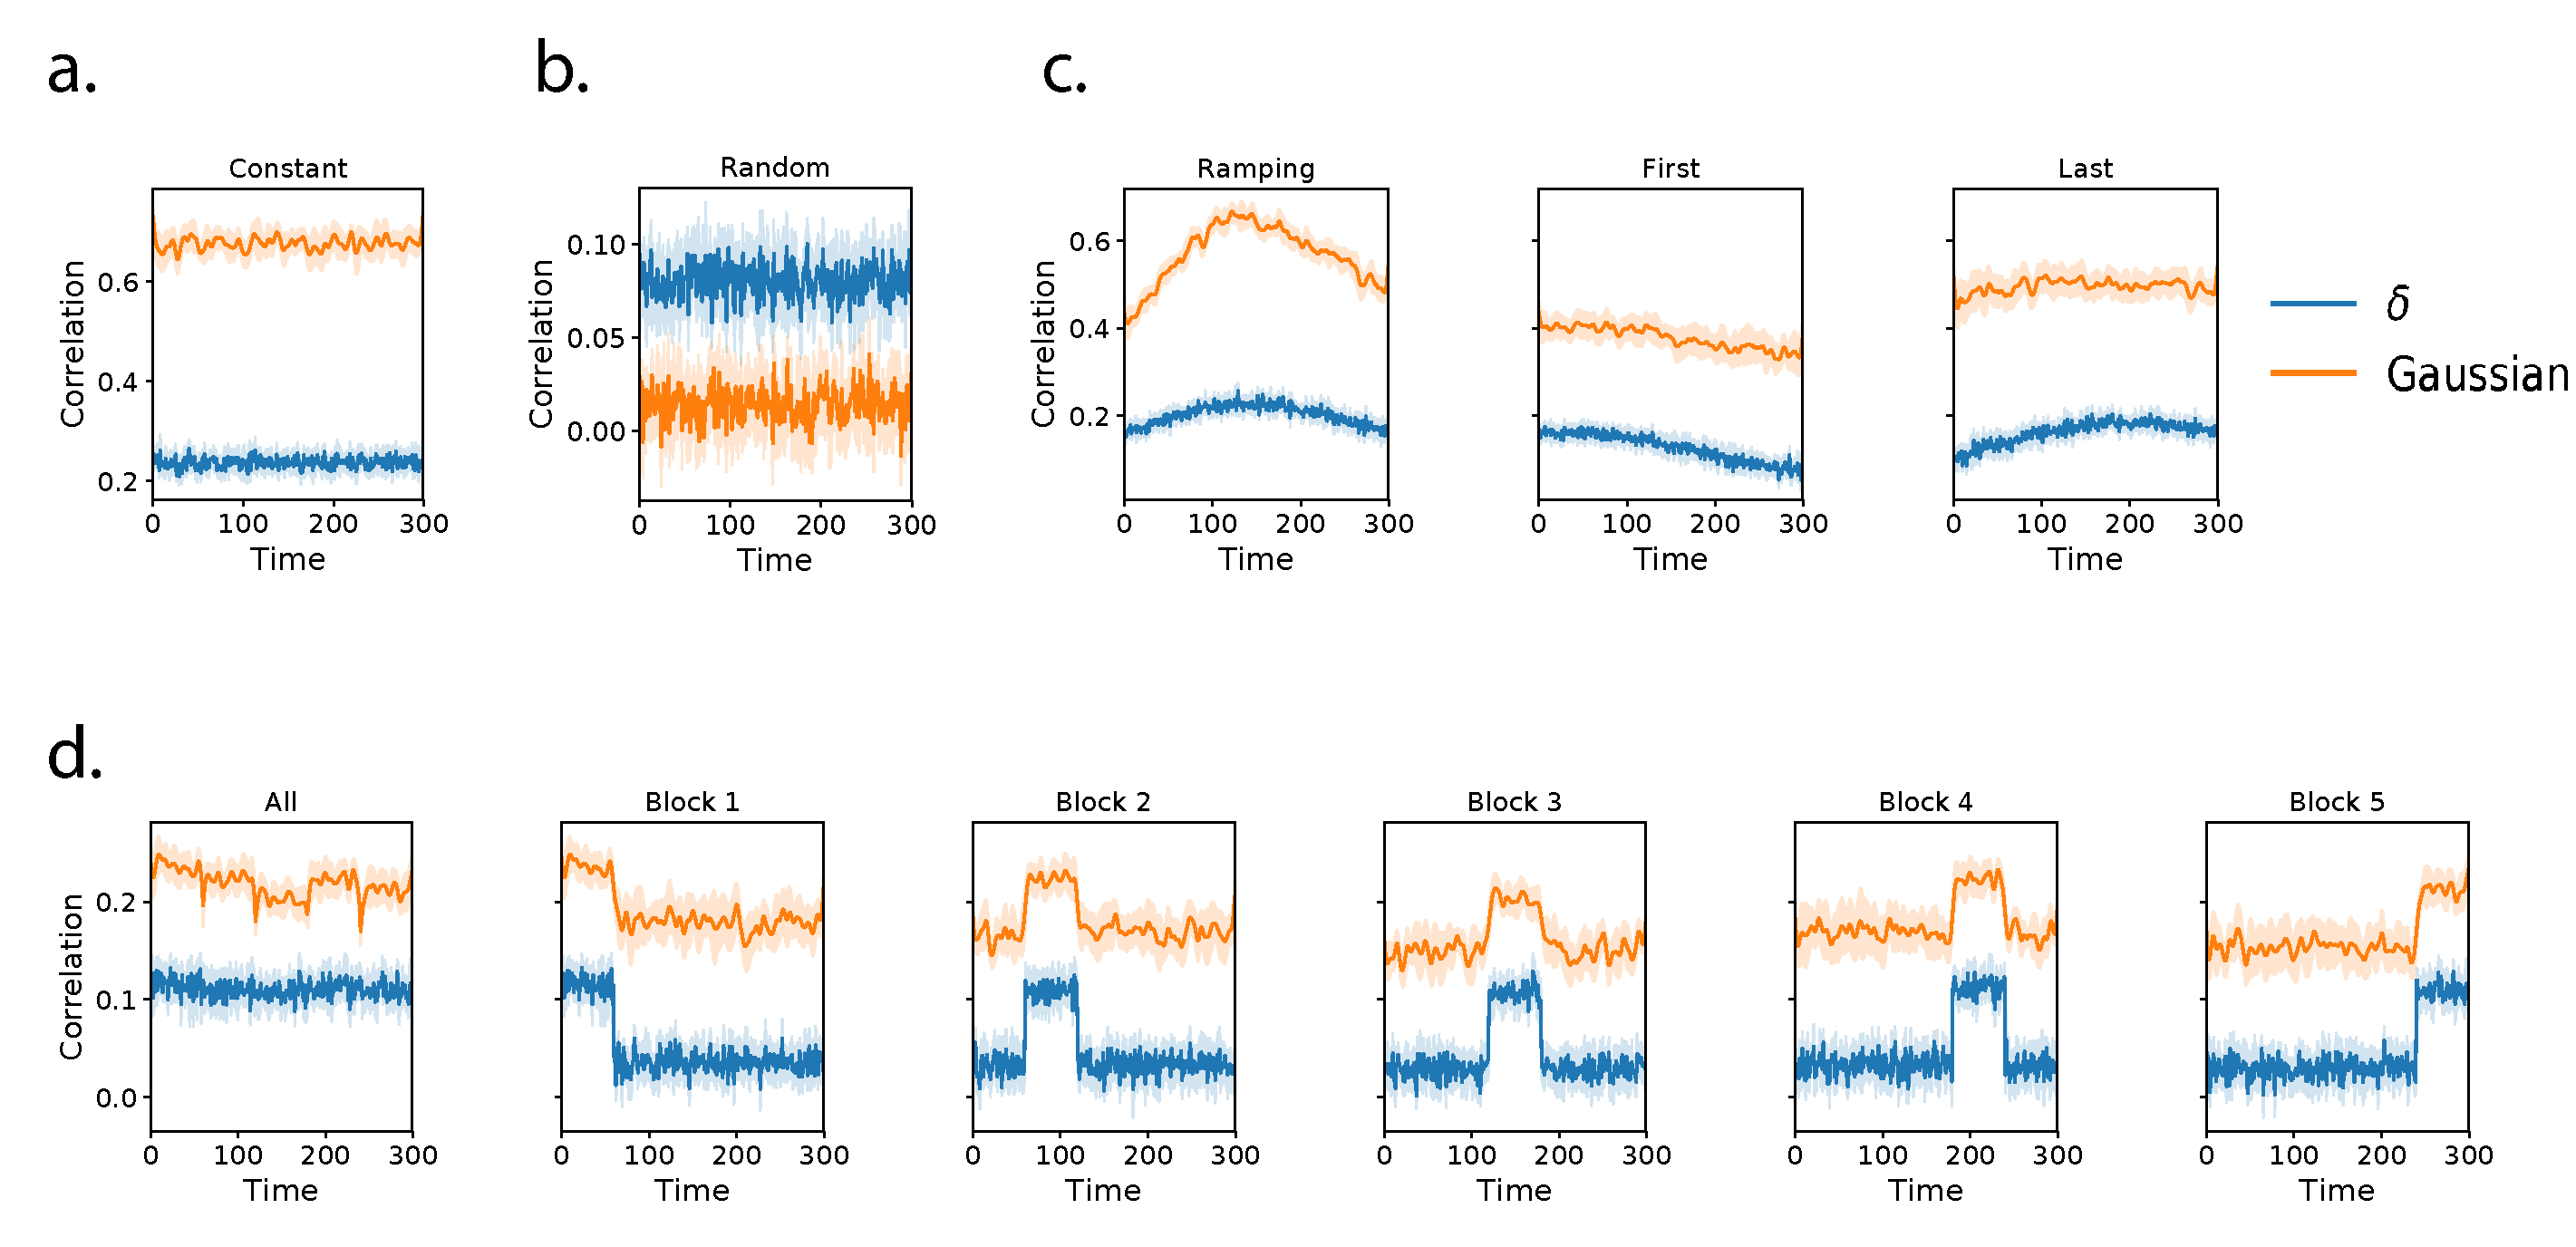
\includegraphics[width=\textwidth]{figs/synthetic_data.pdf}
  \caption{\textbf{Dynamic correlation recovery with synthetic data. } Using synthetic data containing different
    underlying correlational structure,
   we test how well we can recover dynamic correlation matrices using
   different kernels when compared to groud truth.  We compare the results using a delta kernel
   with averaged results from several kernels (Gaussian, Laplace, and
   mexican hat) and several widths (5, 10, 20, and 50).  We plot recovery using of datasets containing the
    following underlying structure:
    \textbf{a. Constant. b. Random. c. Ramping.  d. Block.}}
  \label{fig:synthetic_data}
\end{figure}

To assess the performance of dynamic correlation recovery using
timecorr, we varied width the kernel and the specific structure of the
data. We applied timecorr, using delta and gaussian kernels
Fig.~\ref{fig:weights}) to each of the following  
synthetic datasets: constant, random, ramping, and block.  We then correlated each recovered
correlation matrix with the ground truth. 

For the constant synthetic dataset, a gaussian kernel (width=10)
outperformed the delta kernel (Fig.~\ref{fig:synthetic_data},  a.).  This is in contrast with the random
synthetic dataset, for which the delta kernel best captures the
rapidly changing structure (Fig.~\ref{fig:synthetic_data},  b.). For
the ramping synthetic dataset, the slow changing strucutre within the
data is best
captured by the gaussian kernel and the best recovery occurs in the
middle (Ramping, Fig.~\ref{fig:synthetic_data},
c.). In addition to comparing the timecorr recovered correlation
matrices to the ground truth, we
further compared the ramping recovered correlation matrices to only the first random covariance matrix $K_{1}$
(First, Fig.~\ref{fig:synthetic_data},  c.) and to only the last
random covariance matrix $K_{2}$ (Last, Fig.~\ref{fig:synthetic_data},
c.), both of which perform best at the beginning and end respectively.

Similary for the block sythetic dataset, we compared the timecorr
recovered correlation matrices to the ground truth as well as to each
block-specific covariance matrix (Block 1-5,
Fig.~\ref{fig:synthetic_data},  d.).  Although the structure is
changing by block, the gaussian kernel once again outperforms the
delta kernel.  Performance does however drop near even boundaries for
when using the gaussian kernel. 


\subsubsection*{Neuroimaging dataset~\citep{SimoEtal16}}
For our decoding analysis, we used HTFA-derived node activities
~\cite{MannEtal18} from fMRI data collected as participants listened
to an audio recording of a story (intact condition; 36 participants),
listened to time scrambled recordings of the same story (17
participants in the paragraph-scrambled condition listened to the
paragraphs in a randomized order and 36 in the word-scrambled
condition listened to the words in a randomized order), or lay resting
with their eyes open in the scanner (rest condition; 36
participants). We sought to demonstrate how higher-order correlations
may be used to examine dynamic interactions of brain patterns in
(real) multi-subject fMRI datasets. This story listening dataset was
collected as part of a separate study, where the full imaging
parameters, image preprocessing methods, and experimental details may
be found~\citep{SimoEtal16}. The dataset is available at
\href{url}{http://arks. princeton.edu/ark:/88435/dsp015d86p269k}.

\begin{figure}
  \centering
  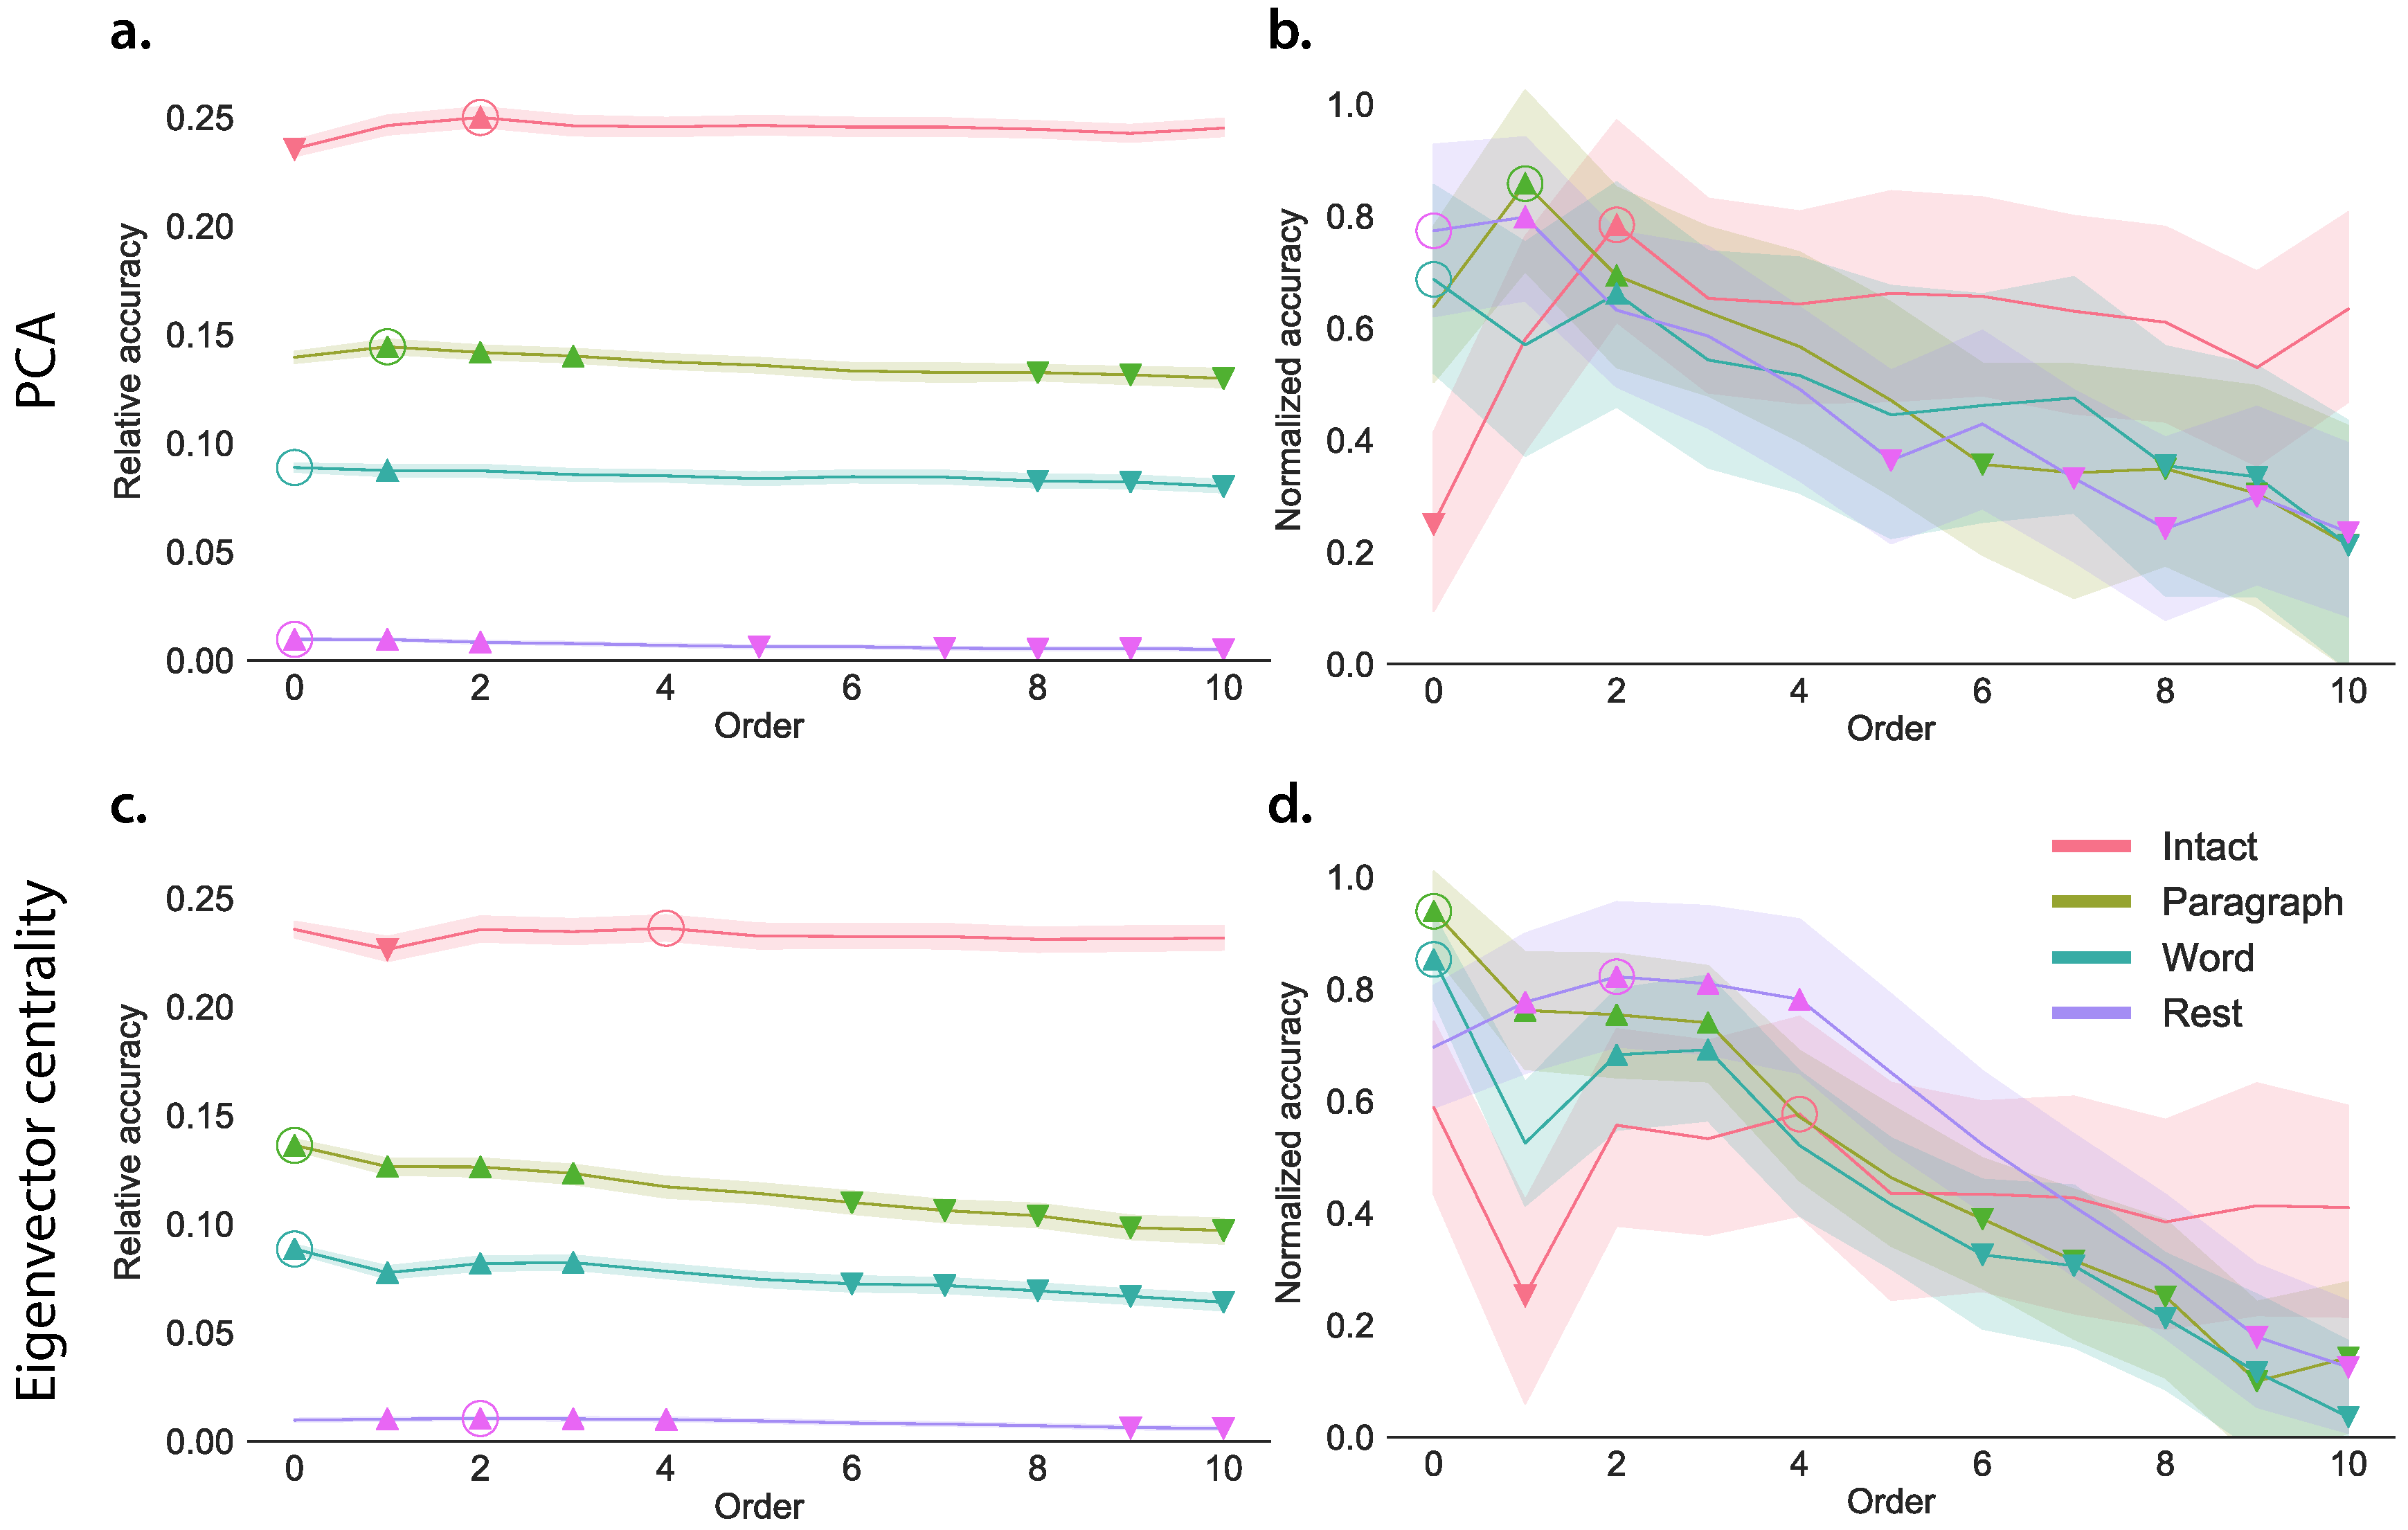
\includegraphics[width=\textwidth]{figs/decode_level.pdf}
  \caption{\textbf{Decoding by order.
      a.\&d. Relative decoding accuracy by order.} Ribbons of each
    color display cross-validated decoding performance averaged over
    all parameters for each condition (intact, paragraph, word,
    and rest) using PCA (a.) or eigenvector centrality (d.) to
    approximate correlations. Decoders were trained using increasingly more
    higher-order information and this ribbons are displayed relative
    to chance at 0. The red dots indicates
    maximum decoding accuracy for each condition. \textbf{b.\&e. Z-transformed decoding accuracy
      by order.}  We Z-transformed the decoding accuracy by order to better
    visualize the order with the maximum decoding accuracy for each
    condition using PCA (b.) or eigenvector centrality (e.) to
    approximate correlations. \textbf{c.\&f. Optimized weights.} Bar heights indicate the
    optimized mixing paramete $\phi$ of each contributing order up to
    and including the order with the maximum
    decoding accuracy for each contributing order using PCA (c.) or eigenvector centrality (f.) to
    approximate correlations.
  For the order with maximum decoding accuracy by condition, we show
  barplots of the optimized weights $\phi$  for each contributing
  order.}
  \label{fig:decoding_level}
\end{figure}


We next evaluated if our model of high-order correlations in brain activity can capture cognitively relevant brain patterns. We performed a decoding analysis, using cross validation to estimate (using other participants’ data) which parts of the story each weighted-mixture of higher-order brain activity pattern corresponded to (see \textit{Materials and methods}). We note that our primary goal was not to achieve perfect decoding accuracy, but rather to use decoding accuracy as a benchmark for assessing whether different neural features specifically capture cognitively relevant brain patterns.

Separately for each experimental condition, we divided participants
into two groups. For the zeroth order, we computed the mean factor
activity for each group.  For all subsequent orders up to the tenth
order, we computed the mean approximated dynamic ISFC of factor
activity for each group (see \textit{Materials and methods}), and
combined in a weighted mixutre with all previous orders
(i.e. cross-validation for the second
order contained a weighted-mixture of zeroth, first, and second order
(Fig.~\ref{fig:decoding_level}, c.\&f.).  For
each order, we correlated the group 1 activity patterns with group 2
activity patterns.  We then subdivided the group 1 to obtain an
optimal weighting parameter for each order’s correlation matrix using
the same cross validation method. We used the optimal weighting
parameters to obtain a weighted-mixture (see \textit{Materials and methods}) of each order’s correlation
matrix. Using these correlations, we labeled the group 1 timepoints
using the group 2 timepoints with which they were most highly
correlated; we then computed the proportion of correctly labeled group
1 timepoints. (We also performed the symmetric analysis whereby we
labeled the group 2 timepoints using the group 1 timepoints as a
template.) We repeated this procedure 100 times (randomly re-assigning
participants to the two groups each time) to obtain a distribution of
decoding accuracies for each experimental condition. There were 272
timepoints for paragraph condition, 300 timepoints for intact and word
conditions, and 400 timepoints for rest condition,  so chance
performance on this decoding test is was $\frac{1}{272}$,
$\frac{1}{300}$, and $\frac{1}{400}$ respectively.
 
We repeated this process for each set of parameters, varying kernel
type and width, and averaged over the reduction technique used to
approximate the higher-order correlations (PCA Fig.~\ref{fig:decoding_level},  a.-c. and eigenvector
centrality Fig.~\ref{fig:decoding_level},  d.-f.).  Since there is no ground truth in these analyses, and we did not know
which parameters best capture the data, we instead report a robustness
search by averaging over the parameters and reporting which results
consistently showed up across all parameters.
\begin{figure}
  \centering
  \includegraphics[width=\textwidth]{figs/brain_plots.pdf}
  \caption{\textbf{Average correlations by order for the intact listening condition.} Using eigenvector
    centrality to approximate higher-order correlations for the
    intact, paragraph scrambled, word scrambled, and rest condition.
    We plot the
    strongest 50\% absolute value
    mean correlation for \textbf{a.-d. first order, e.-h. second order,
      i.-l. third order, and m.-p. fourth order }, representing the degree of agreement by
    location pair over time.  To demonstrate how this method is
    computationally scalable, we also approximated
    \textbf{a.-d. fifteenth order} dynamic correlation, which would be
    possible to compute using conventional methods since it would require more bits to represent the solution than there are molecules in the universe.}
  \label{fig:brain_plots}
\end{figure}

The two methods used to approximate the higher-order correlations (PCA Fig.~\ref{fig:decoding_level},  a.-c. and eigenvector
centrality Fig.~\ref{fig:decoding_level},  d.-f.) capture different
facets of the activity patterns.  Using PCA, the higher-order
correlations are all linked to the original activity patterns, whereas
eigenvectory centrality breaks the immediate link with specific brain
areas and instead characterizes the position of the nodes in the
network that are similar over time.

We found for both PCA and eigenvector centrality, during the intact condition in the
experiment, classifiers that incorporated higher-order correlations
yielded consistently higher accuracy than classifiers trained only on
lower-order patterns (Fig.~\ref{fig:decoding_level},  a.\&d.).  We plot
the average correlations for up to the fourth order for the intact
condition (Fig.~\ref{fig:brain_plots}) representing the degree of
agreement by location pair over time.  By
contrast, we found that incorporating higher-order (greater than first
order) correlations did
not further improve decoding accuracy for the other listening
conditions or rest condition.  This suggests
that the cognitive processing that supported the most cognitively rich
condition
involved higher-order network dynamics. 




%%%%%%%%%%%%%%%%%%%%%%%%%%%%%%%%%%%%%%%
\section*{Discussion}

\begin{figure}
  \centering
  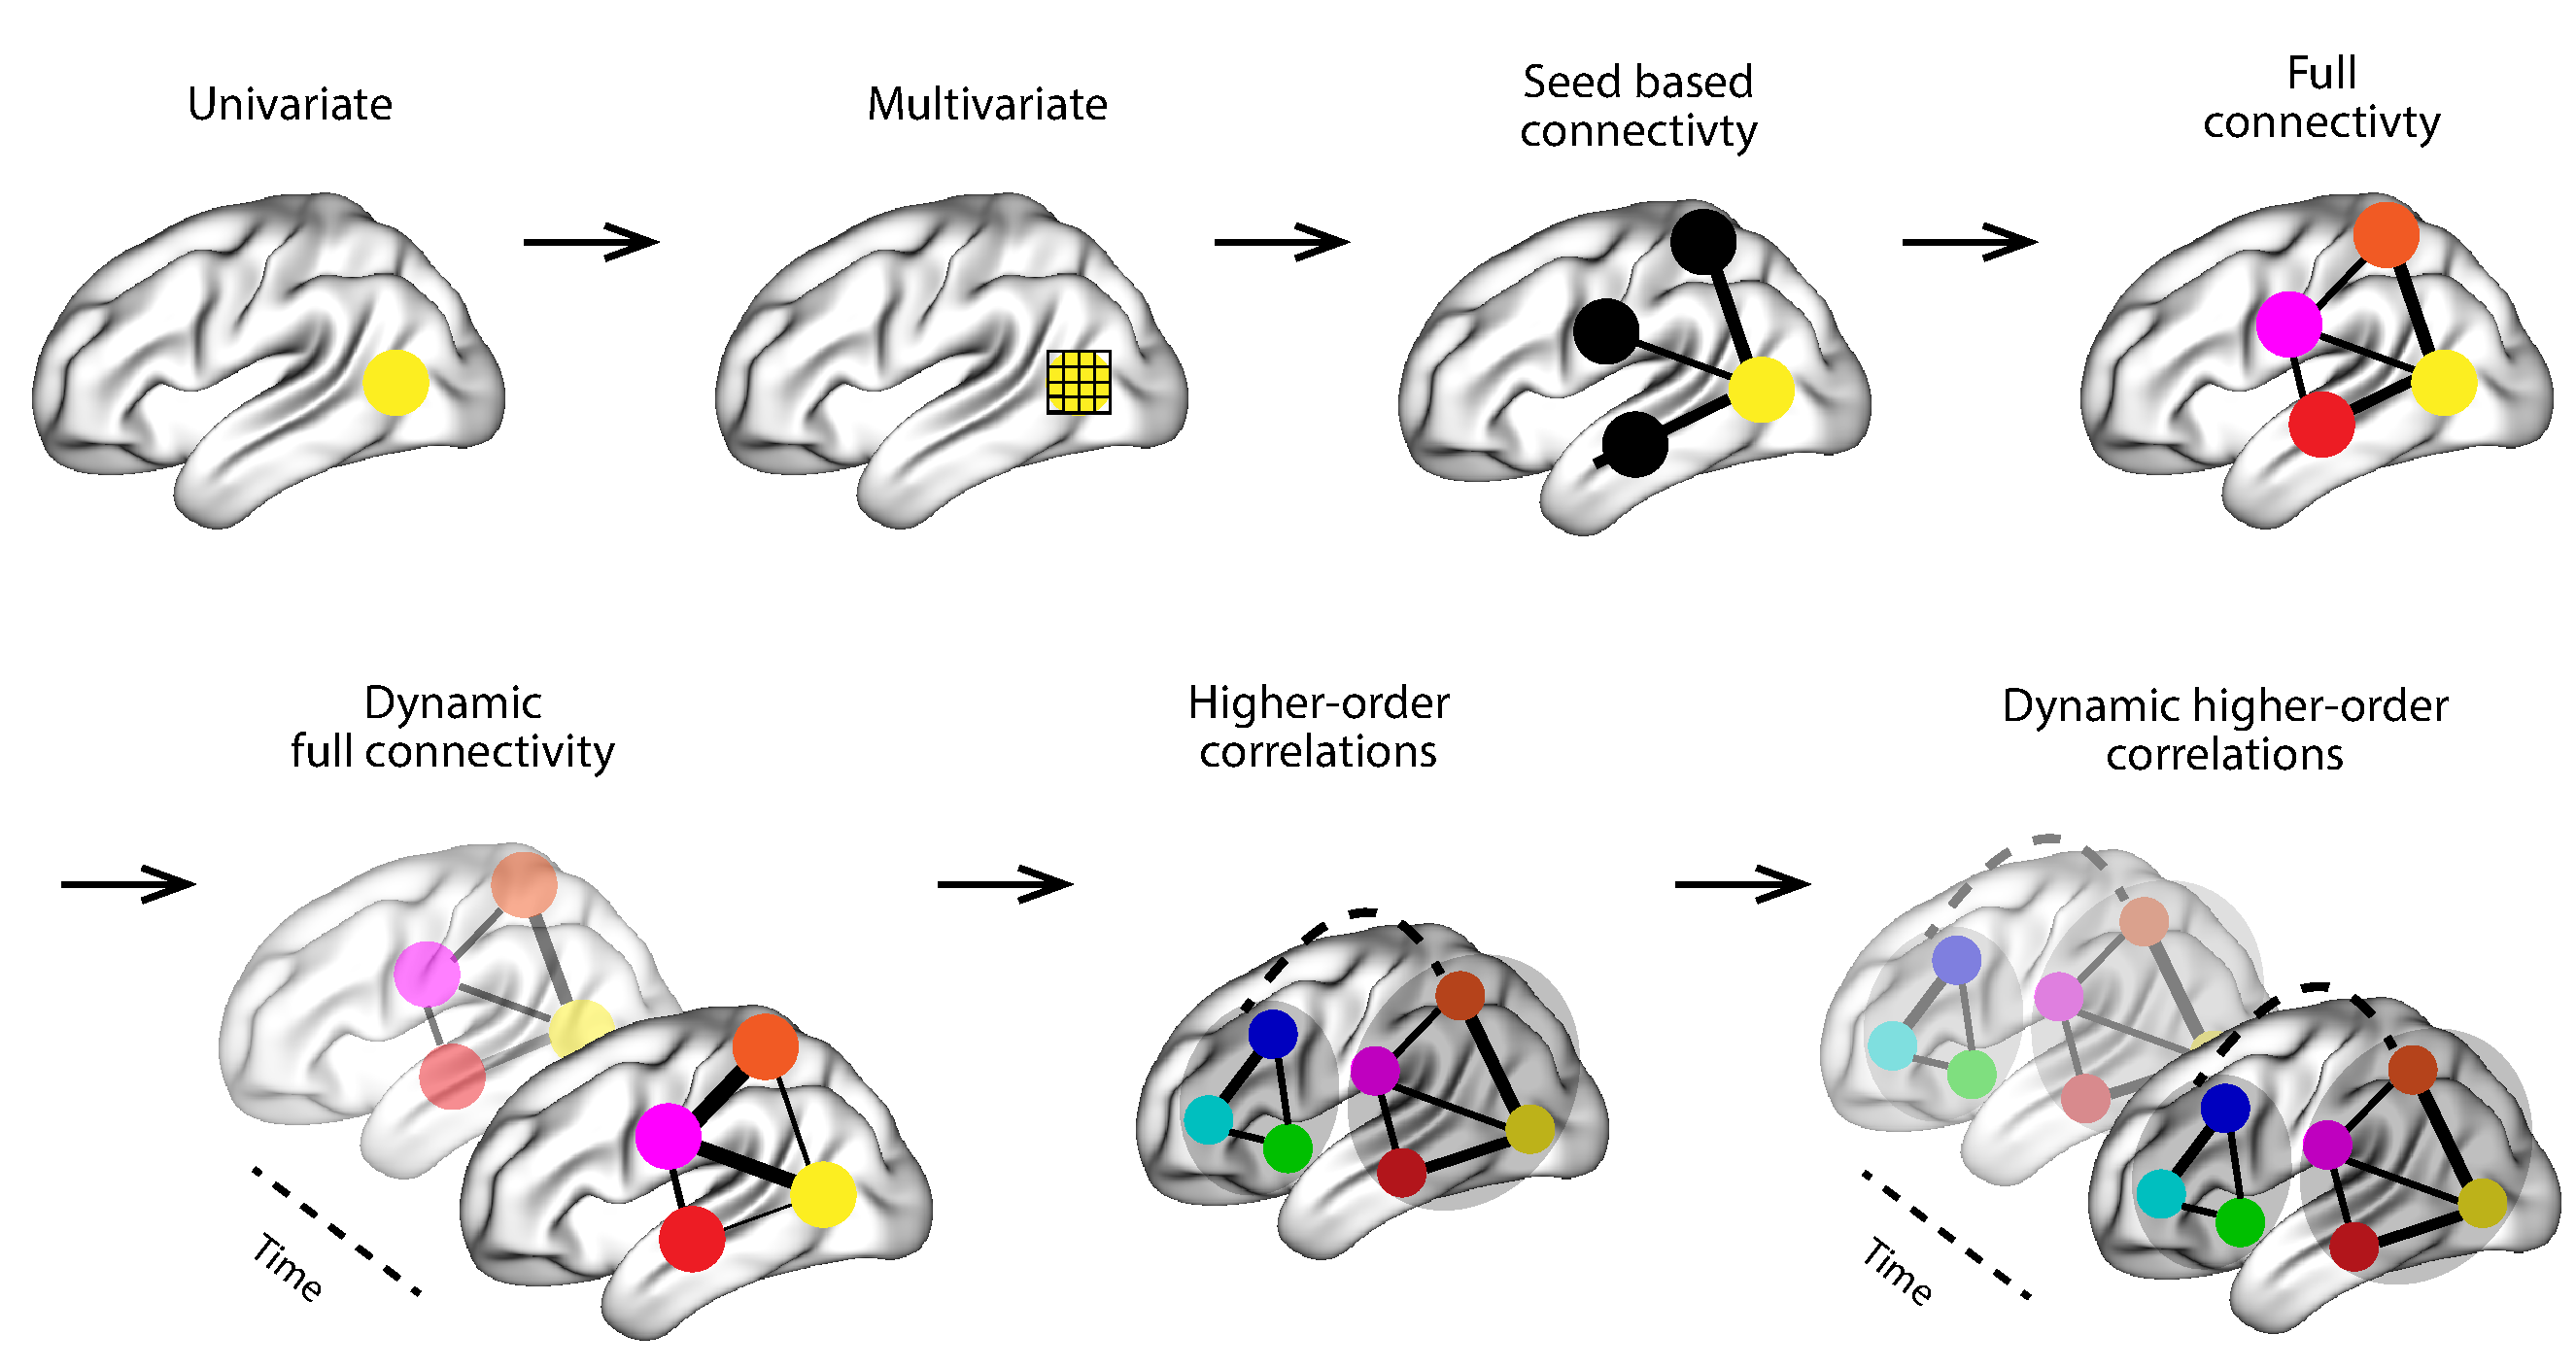
\includegraphics[width=\textwidth]{figs/direction_of_field.pdf}
  \caption{\textbf{Direction of the field (adapted from~\citep{Turk13}).} The evolution of fMRI analyses started with
    univariate activation, which refers to
    the average amplitude of BOLD activity evoked by events of an
    experimental condition. Next, multivariate classifiers are trained
    on patterns of activation across voxels to decode distributed
    representations for specific events. The next, resting
    connectivity, is the temporal correlation of one or more seed
    regions with the remainder of the brain during rest. Additionally,
    task-based connectivity examines how these correlations differ by
    cognitive state. Following this increasing trajectory of
    increasing complexity, full connectivity considers all pairwise
    correlations in the brain, most commonly at rest.  Next, dynamic
    full connectivity considers how full connectivity changes over
    time. Continuing this line of reasoning, we expect higher-order network dynamics might provide even richer insights into the neural basis of cognition.}
  \label{fig:direction_of_field}
\end{figure}



Based on prior work ~\citep{DemeEtal19} and following the direction of the field ~\citep{Turk13} we think our thoughts might be encoded in
dynamic network patterns, and possibly higher order network
patterns (Fig.~\ref{fig:direction_of_field}). We sought to test this hypothesis by developing an approach
to inferring high-order network dynamics from timeseries data. 

One challenge in studying dynamic interactions is the
computational resources required to calculate higher-order correlations. 
We developed a computationally tractable model of network dynamics (Fig.~\ref{fig:methods_fig}) that takes in a feature
timeseries and outputs approximated first-order dynamics (i.e.,
dynamic functional correlations), second-order dynamics
(reflecting homologous networks that dynamically form and disperse),
and higher-order network dynamics (up to tenth-order dynamic
correlations).

We first validated our model using synthetic data, and explored how
recovery varied with different underlying data structures and kernels.   We then 
applied the approach to an fMRI dataset
~\citep{SimoEtal16} in which participants listened to an audio
recording of a story, as well as scrambled versions of the same story
(where the scrambling was applied at different temporal scales).  We
trained classifiers to take the output of the model and decode the
timepoint in the story (or scrambled story) that the participants were
listening to. We found that, during the intact listening condition in the
experiment, classifiers that incorporated higher-order correlations
yielded consistently higher accuracy than classifiers trained only on
lower-order patterns (Fig.~\ref{fig:decoding_level},  a.\&d.).  By contrast, these
higher-order correlations were not necessary to support decoding the other
listening conditions and (minimally
above chance) during a control rest condition.  This suggests
that the cognitive processing that supported the most cogntively rich listening conditions
involved second-order (or higher) network dynamics.

Although we found decoding accuracy was best when incorporating
higher-order network dynamics for all but rest
  condition, it is unclear if this is a product of the brain or the
  data collection technique.  It could be that the brain is
  second-order or it could be that fMRI can
  only reliably give second-order interactions. Exploring this method
  with other data collection technique will be important to
  disentangle this question.



  \subsection*{Concluding remarks}

How can we better understand how brain patterns change over
time? How can we quantify the potential network dynamics that might be
driving these changes? One way to judge the techniques of the future is
to look at the trajectory of the fMRI field so far has taken so far
(Fig.~\ref{fig:methods_fig}).  The field started with 
univariate activation, measuring the average activity for each voxel.
Analyses of multivariate activation followed, looking at spatial patterns of
activity over voxels. Next, correlations of activity were explored, first
with measures like resting connectivity that take temporal correlation
between a seed voxel and all other voxels then with full connectivty
that measure all pairwise correlations.  Additionally, this path of increasing
complexity also moved from static to dynamic measurements.  One
logical next step in this trajectory would be dynamic higher-order
correlations. We have created a method 
to support these calculations by scalably approximating dynamic higher-order
correlations.  

\section*{Acknowledgements}
We acknowledge discussions with Luke Chang, Hany Farid, Paxton
Fitzpatrick, Andrew Heusser, Eshin Jolly, Qiang Liu, Matthijs van der
Meer, Judith Mildner, Gina Notaro, Stephen Satterthwaite, Emily
Whitaker, Weizhen Xie, and Kirsten Ziman. Our work was supported in
part by NSF EPSCoR Award Number 1632738 to J.R.M. and by a sub-award
of DARPA RAM Cooperative Agreement N66001-14-2-4-032 to J.R.M.  The
content is solely the responsibility of the authors and does not
necessarily represent the official views of our supporting
organizations.

\section*{Author contributions}
Concept: J.R.M.  Implementation: T.H.C., L.L.W.O., and
J.R.M.  Analyses: L.L.W.O and J.R.M.

\bibliographystyle{apacite}
\bibliography{CDL-bibliography/memlab}

\end{document}


